%\chapter{涵道风扇式无人机的控制分配问题}
\chapter{涵道风扇式无人机的自抗扰控制}
%
通过上一章的建模分析,从涵道飞行器的动力学模型可以看出,涵道无人机在飞行过程中受到复杂气动力和气动力矩的影响。对于姿态控制而言,不仅受舵面的驱动力矩作用,还受固定气动面的平衡扭矩、风扇扭矩、陀螺力矩、气动俯仰力矩的作用。这些力矩难以得到其解析形式,但却极大的影响飞机飞行性能。比如,飞机在进行高度控制的过程中需要改变螺旋桨转速,但这同时将因为转速的改变而直接改变系统受到的陀螺力矩、平衡扭矩、风扇扭矩。在存在外扰动时,如果不合理的转换控制力矩到各个舵面偏转角,那么舵面提供的驱动力矩很可能不能抵消这些扰动,从而使系统发散。要使姿态控制更为稳健,首先需要估计这些扰动,对扰动进行补偿之后将控制量转换成舵面偏转角。本节将介绍一种扰动抑制控制算法,将其改进后应用到涵道无人机的姿态控制中。
\section{从PID控制到自抗扰控制}
PID控制器根据系统输入和参考输入的误差进行控制,用误差来消除误差,而不需要知道系统的数学模型。因其参数调节过程简单,参数物理意义明确,在工程实践中得到广泛应用。然而随着科技的发展,工业界对控制器性能的要求越来越高,PID控制的缺点日益明显,主要有:
\begin{enumerate}
	\item PID控制律是基于参考信号与系统输出的误差进行计算的。物理系统的输出通常光滑的,但输入参考信号往往是不光滑的阶跃信号。这一矛盾导致误差的初始值往往比较大,进而使得系统受到较大的冲击产生超调和震荡。为了减小超调,通常是减小控制器增益,但又会使得调节时间变长。即PID控制器存在快速性和超调之间的矛盾。
	\item 实际系统中噪声的存在使得微分器难以实现。
	\item PID控制律是误差的比例、积分、微分的线性组合,组合方式并非最优。
	\item 积分器虽然可以消除静态误差,但会产生积分饱和导致大超调和震荡次数的增加,使系统不稳定。 
\end{enumerate}

针对PID控制的不足,ADRC做了如下改进:
\begin{enumerate}
	\item 为参考输入安排过渡过程:根据系统的阶次安排合适的过渡过程,解决超调和快速性之间的矛盾。使得误差反馈增益的取值范围更大,同时给定的反馈增益能适用于更多的系统,控制器鲁棒性增强。
	\item 提取微分信号:设计非线性微分跟踪器来提取参考输入的微分,降低噪声的影响。同时还设计扩张状态观测器提取反馈信号的微分。
	\item 非线性误差反馈:对误差的比例、微分应用非线性组合构建控制量,得到比线性组合更好的效果。
	\item 估计总和扰动:应用ESO实时估计系统的总和扰动,在控制律中包含扰动补偿,避免了积分反馈的副作用,同时提高了系统抗干扰能力。
\end{enumerate}
\section{自抗扰控制器原理}
自抗扰控制器由跟踪微分器(TD)、扩张状态观测器(ESO)以及非线性误差反馈(NLESF)组成。自抗扰控制技术不依赖于对象的数学模型,通过扩张状态观测器实时估计出包含系统内部模型不确定性和外部扰动不确定性的总扰动,通过动态补偿的方法,将实际系统补偿为积分串联型的标准结构。ADRC的收敛性最初由文献\parencite{HanJingQing_2008}给出分析。近年来,郭宝珠等人给出了更严格的数学证明,在文献\parencite{Guo_2010,Guo_2011b,Guo_2011c,Guo_2011d}给出了跟踪微分器的收敛性证明。文献\parencite{Guo_2011,Guo_2011a,Guo_2012,Zhao_2016}给出了扩张状态观测器的收敛性证明,文献\parencite{Guo_2013,Zhao_2016a,Guo_2013,Guo_2012a}分析了ADRC闭环系统的收敛性。本节将逐一介绍其原理,并不加证明地给出几条收敛性定理。
\subsection{跟踪微分器}
物理系统通常有一定的惯性,其状态一般不会突变,而参考输入却可能会是突变信号。因此在跟踪问题中,要求系统跟随突变信号是不合理的。利用跟踪微分器产生参考指令的过渡过程和提取微分信号,使得系统初始误差更为合理。借助微分跟踪器,系统可以使用更大的控制增益,可提高系统快速性。

可设计如下形式的二阶跟踪微分器
\begin{align}
\left\{\begin{array}{l}
\dot{v}_{1}(t)=v_{2}(t) \\
\dot{v}_{2}(t)=R^{2}\left(-\zeta_{1}\left[v_{1}(t)-v_c(t)\right]^{\alpha}-\zeta_{2}\left[\dfrac{v_{2}(t)}{R}\right]^{\beta}\right)
\end{array}\right.	\label{eq_sec_TD}
\end{align}
其中$ [r]^{\alpha}=\operatorname{sign}(r)\left|r\right|^{\alpha} $,且
\begin{align}
\zeta_{1}, \zeta_{2}>0, \alpha=\dfrac{b-1}{a}, \beta=\dfrac{b-1}{b}, a=b+1, b>1	\label{eq_para_sec_TD}
\end{align}
若选取适当参数,则TD的状态$ {v}_{1}(t) $即为所安排的过渡过程,$ v_{2}(t) $为参考输入$ v_c(t) $的微分信号。其收敛性可由如下定理给出\cite{Guo_2011b}:
\begin{theorem}
	如果待处理信号满足$ \sup\limits_{t \in[0, \infty ) }\left|v^{(i)}_c(t)\right|<\infty, i=1,2.$则跟踪微分器\eqref{eq_sec_TD}是收敛的,即对于任意的初始值和$\forall T_1 >0 $, $\exists R_0 >0 $使得对$\forall R>R_0 $及$ t>T_1 $,有
	\begin{align}
	\left|v_{1}(t)-v_c(t)\right| \leq M_{1}\left(\dfrac{1}{R}\right)^{\beta {\frac{1-\gamma}{\gamma}}}, \quad\left|v_{2}(t)-\dot{v}_c(t)\right| \leq M_{2}\left(\dfrac{1}{R}\right)^{\beta \frac{1-\gamma}{\gamma}-1}
	\end{align}
	其中$\gamma=\frac{l-1}{l}, l>\max \{1, a, b\}$,$ M_1 $、$M_2$是依赖于初始值的常数,$ \alpha $、$\beta$是满足式\eqref{eq_para_sec_TD}的参数。		\label{the_sec_TD}
\end{theorem}
\subsection{扩张状态观测器}
自抗扰控制的核心是设计扩张状态观测器,对系统未建模动态和外部扰动进行估计。通过在系统中实时补偿该“总和扰动”,使对象模型变成“积分器串联型”线性系统。考虑更具一般性的$ n $阶的情况,针对如下系统
\begin{align}\left\{\begin{array}{l}
x^{(n)}(t)=f\left(t, x(t), \dot{x}(t), \ldots, x^{(n-1)}(t)\right)+w(t)+bu(t) \\
y(t)=x(t)
\end{array}\right.	\label{eq_sys}
\end{align}
其中$ w(t) $为系统的外部扰动,简记为$ w $,$ f\left(t, x_{1}(t), x_{2}(t), \ldots, x_{n}(t)\right) $为系统内部不确定函数,简记为$ f $。将上式改写为
\begin{align}\left\{\begin{array}{l}
\dot{x}_{1}(t)=x_{2}(t),\quad
\dot{x}_{2}(t)=x_{3}(t)  \\
\vdots \\
\dot{x}_{n}(t)=f\left(t, x_{1}(t), x_{2}(t), \ldots, x_{n}(t)\right) +w(t)+bu(t)	\\
y(t)=x_{1}(t)
\end{array}\right.	\label{eq_n_diff}
\end{align}
并将$ f+w $扩充为新的状态,可设计扩张状态观测器\cite{Guo_2012}
\begin{align}\left\{\begin{array}{l}
\dot{\hat{x}}_{1}(t)=\hat{x}_{2}(t)+\varepsilon^{n-1} g_{1}\left(\dfrac{y(t)-\hat{x}_{1}(t)}{\varepsilon^{n}}\right)\\[3mm]
\dot{\hat{x}}_{2}(t)=\hat{x}_{3}(t)+\varepsilon^{n-2} g_{2}\left(\dfrac{y(t)-\hat{x}_{1}(t)}{\varepsilon^{n}}\right) \\
\vdots \\
\dot{\hat{x}}_{n}(t)=\hat{x}_{n+1}(t)+g_{n}\left(\dfrac{y(t)-\hat{x}_{1}(t)}{\varepsilon^{n}}\right)+bu(t) \\[3mm]
\dot{\hat{x}}_{n+1}(t)=\dfrac{1}{\varepsilon} g_{n+1}\left(\dfrac{y-\hat{x}_{1}(t)}{\varepsilon^{n}}\right)
\end{array}\right.  	\label{eq_NLESO}
\end{align}
使观测器状态$ \hat{x}_i,i=1,2,\dots,n+1 $分别收敛于系统状态$ x_1,x_2,\dots,x_n $以及$ f+w $。该观测器的收敛性结论需要如下几个假设\cite{Guo_2012,Guo_2011}:
\begin{assumption}
	函数$ f $,$ w $对所有自变量都是连续可微的,且满足
	\begin{align}|u|+|f|+|\dot{w}|+\left|\dfrac{\partial f}{\partial t}\right|+\left|\dfrac{\partial f}{\partial x_{i}}\right| \leq c_{0}+\sum_{j=1}^{n} c_{j}\left|x_{j}\right|^{k}\end{align}
	其中$c_{j}, j=0,1, \cdots, n$是正实数, $ k $是正整数。	\label{H1}
\end{assumption}	
\begin{assumption}
	外部扰动$w$和式\eqref{eq_n_diff}所示系统的解满足
	\begin{align}
	|w|+\left|x_{i}(t)\right| \leq \bm{B}
	\end{align}
	其中$ B>0 $,$ i=1,2,\cdots,n $,$ t>0 $。	\label{H2}
\end{assumption}
\begin{assumption}
	存在常数$ \lambda_i,i=1,2,3,4 $、$ \alpha $、$ \beta $以及连续的正定函数$ V,W:\mathbb{R}^{n+1} \rightarrow \mathbb{R} $满足下面三个条件
	\begin{enumerate}
		\item $ \lambda_{1}\|\bm{y}\|^{2} \leq V(\bm{y}) \leq \lambda_{2}\|\bm{y}\|^{2}, \quad \lambda_{3}\|\bm{y}\|^{2} \leq W(\bm{y}) \leq \lambda_{4}\|\bm{y}\|^{2} $ 
		\item $ \sum_{i=1}^{n} \frac{\partial V}{\partial y_{i}}\left(y_{i+1}-g_{i}\left(y_{1}\right)\right)-\frac{\partial V}{\partial y_{n+1}} g_{n+1}\left(y_{1}\right) \leq-W(\bm{y}) $ 
		\item $ \left|\frac{\partial V}{\partial y_{n+1}}\right| \leq \beta\|\bm{y}\| $		
	\end{enumerate}
	其中$\bm{y}=[y_{1} \quad y_{2} \quad \ldots \quad y_{n+1}]^{\top}$,$\|\cdot\|$表示$ \mathbb{R}^{n+1} $中的欧几里得范数	\label{H3}
\end{assumption}
\begin{theorem}
	若假设\ref{H1}、\ref{H2}以及\ref{H3}成立,那么有
	\begin{enumerate}
		\item 对于任意给定的$ a>0 $,$ \lim\limits_{\varepsilon \rightarrow 0}\left|x_{i}(t)-\hat{x}_{i}(t)\right|=0 $在$t \in [a, \infty)$上—致地成立	
		\item $ \lim\limits_{t \rightarrow \infty}\left|x_{i}(t)-\hat{x}_{i}(t)\right| \leq O\left(\varepsilon^{n+2-i}\right)  $
	\end{enumerate}
	其中$x_{i}$,$ \hat{x}_{i}$分别为式\eqref{eq_n_diff}所示系统和式\eqref{eq_NLESO}所示ESO的解,$i=1,2, \ldots, n+1$,$ x_{n+1}=f+w$是式\eqref{eq_n_diff}所示系统的扩张状态	\label{the_NLESO}
\end{theorem}
\subsection{非线性误差反馈}
在ADRC控制技术中,延拓了“基于误差来消除误差”的思想。将跟踪微分器得到的跟踪信号以及微分信号与ESO中得到的系统状态的估计信号做差,通过特定的组合产生误差反馈。与PID不同的地方在于,最终的控制量是在误差反馈的基础上添加一个扰动补偿项,将非线性系统线性化。误差反馈使线性化后的系统跟踪给定输入。

以$ n=2 $即二阶系统为例,由上文可知参考输入$ v_c $经过跟踪微分器得到的过渡过程及其微分信号为$ v_1 $、$ v_2 $,ESO估计的系统状态为$ \hat{x}_1 $和$ \hat{x}_2 $,由此定义状态误差
\begin{align}\begin{array}{l}
e_{1}=v_{1}-\hat{x}_{1} \\
e_{2}=v_{2}-\hat{x}_{2}
\end{array}\end{align}
误差反馈定义为$ u_{0}=\Phi (e_1,e_2) $,常见的误差反馈有
\begin{align}
u_{0} &=k_1 e_{1}+k_2 e_{2} \label{eq_LEF}	\\	
u_{0} &=k_{1} fal\left(e_{1}, \alpha_{1}, \delta\right)+k_{2} fal\left(e_{2}, \alpha_{2}, \delta\right)	\label{eq_NLEF}
\end{align}
其中$ 0<\alpha_{1}<1<\alpha_{2} $,且
\begin{align}
fal(e, \sigma, \xi)=
\begin{cases}
|e|^{\sigma} \operatorname{sgn}(e) &  |e|>\xi,\\
e / \xi^{1-\sigma} &  |e| \leq \xi.
\end{cases}\quad \xi >0
\end{align}
结合扩张状态观测器估计到的总和扰动$ z_{3} $,则总的控制律为
\begin{align}
u=\dfrac{u_{0}-z_{3}}{\hat{b}}=\dfrac{1}{\hat{b}}(\Phi (e_1,e_2) -z_{3})
\end{align}
此时式\eqref{eq_sys}所示被控对象对应的闭环系统变为积分串联型系统
\begin{align}\left\{\begin{array}{l}
\dot{x}_{1}=x_{2} \\
\dot{x}_{2}=\Phi(e_1,e_2) \\
y=x_{1}
\end{array}\right.\end{align}
整个闭环系统结构框图如图\ref{fig_ADRC}所示
\begin{figure}[htbp]
	\centering	
	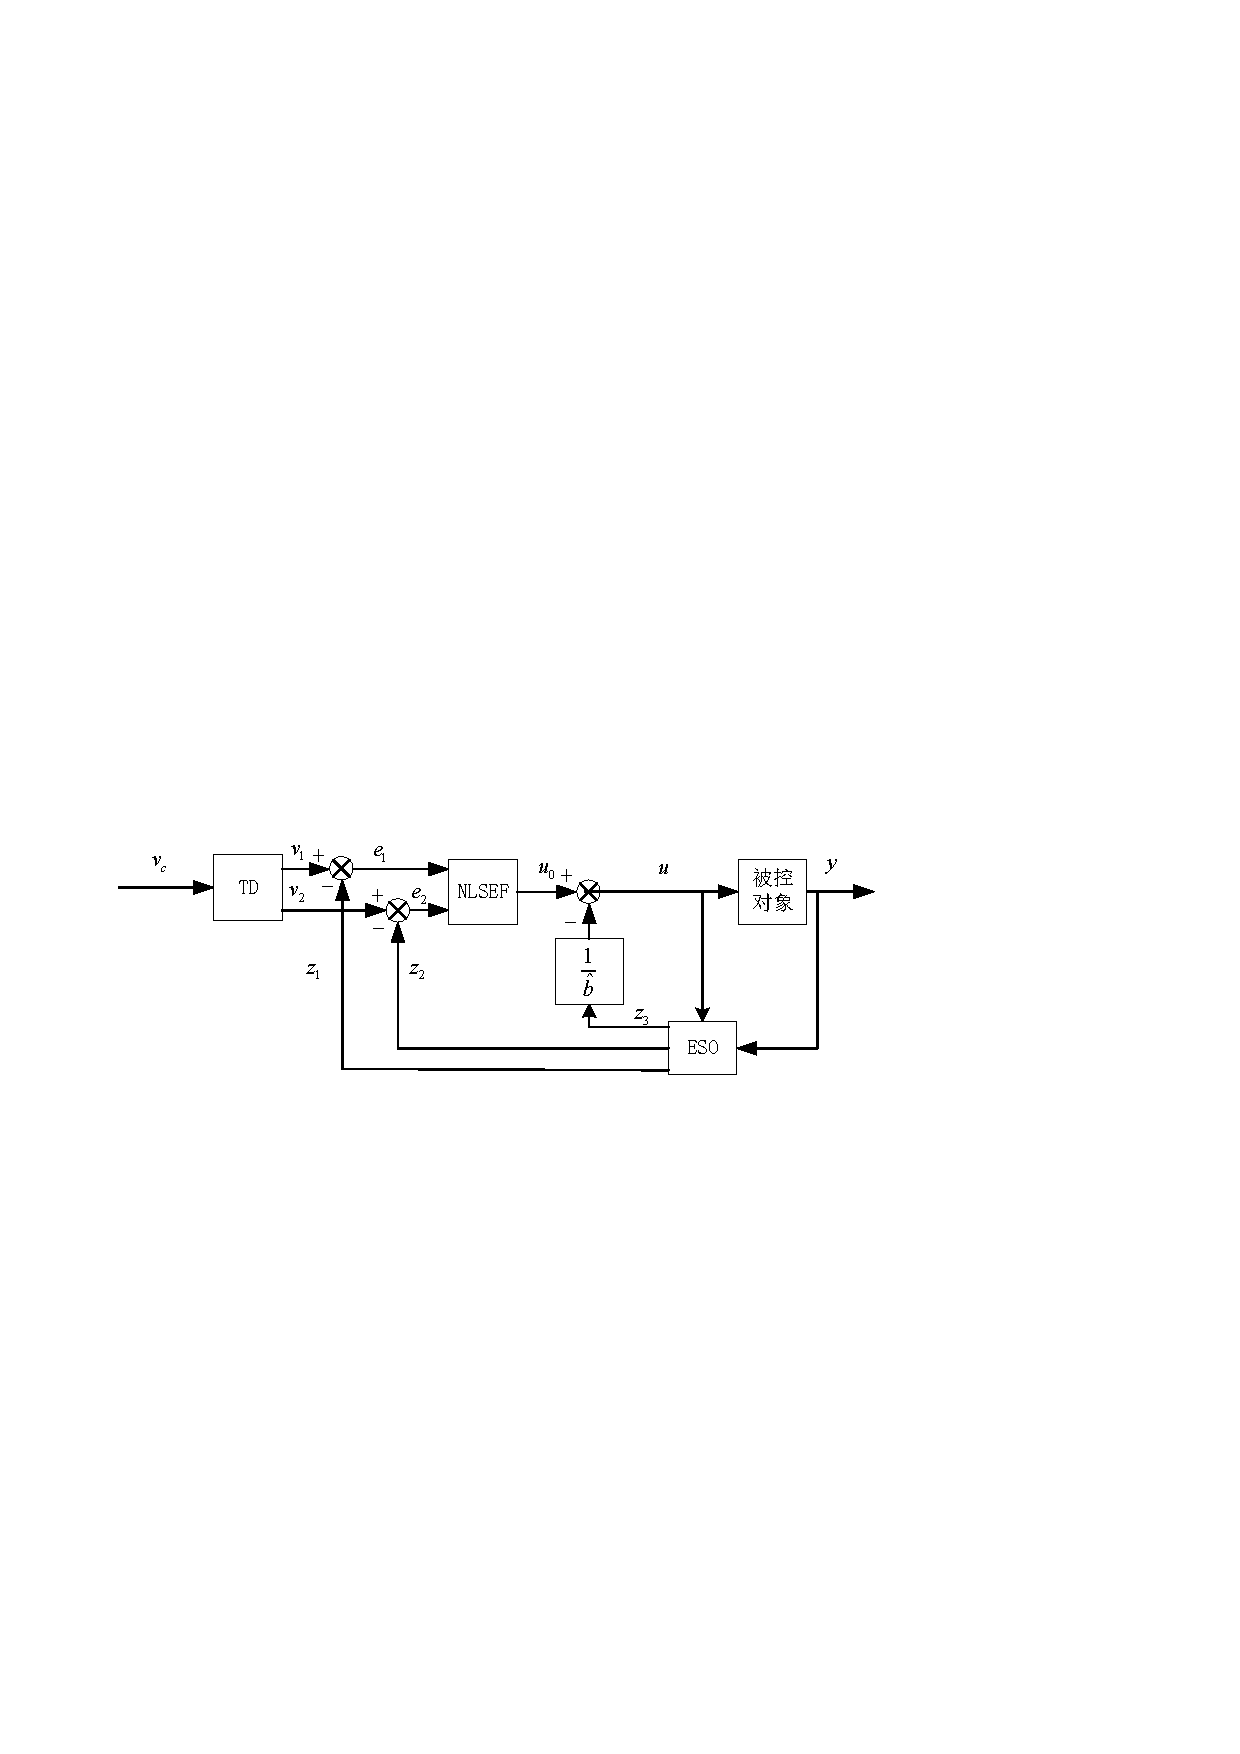
\includegraphics[scale=1]{Fig/Fig_ADRC.pdf}
	\caption{\label{fig_ADRC}自抗扰控制器结构框图}
\end{figure}
\section{自抗扰控制的收敛性}
%闭环系统的稳定性和输入无关,因此分析ADRC闭环系统的稳定性仅考虑在非线性扩张状态观测器\eqref{eq_NLESO}和非线性反馈  eq_h_TD  eq_NLESO 
针对式\eqref{eq_n_diff}所示$ n $阶SISO系统,所设计的ADRC由TD、ESO、NLESF三部分组成,在给出自抗扰控制的收敛性证明之前先简单回顾其主要思想。

%针对式\eqref{eq_n_diff}所示$ n $阶SISO系统,ADRC的目的是使该系统的观测输出$y$跟踪参考之类$v$,同时系统状态$ x_{i}(t) $跟踪参考输入的微分信号$v^{i-1},i=2,\ldots,n$。

假设如下参照系统的零平衡点是全局渐近稳定的
\begin{align}\left\{\begin{array}{l}
\dot{x}_{1}^{*}(t)=x_{2}^{*}(t) \\
\dot{x}_{2}^{*}(t)=x_{3}^{*}(t) \\
\vdots \\
\dot{x}_{n}^{*}(t)=\Phi\left(x_{1}^{*}(t), \ldots, x_{n}^{*}(t)\right), \Phi(0,0, \ldots, 0)=0
\end{array}\right.	\label{eq_ref_sys}
\end{align}
自抗扰控制首先是设计式\eqref{eq_sec_TD}所示跟踪微分器,由参考输入$ v_c $,得到其过渡过程$v_1$及估计到其导数$v_2,v_3,\ldots,v_n$。控制目标是使即$x_i$按照参照系统的状态$ x^*_i $收敛于零的方式收敛于$v_i$。其次设计如式\eqref{eq_NLESO}的扩张状态观测器,得$\hat{x}_1,\hat{x}_2,\ldots,\hat{x}_{n+1}$用以估计系统状态$x_i,i=1,2,\ldots,n$以及扩张状态$x_{n+1}=f+(b-\hat{b}) u$。最后设计如下包含扰动补偿的非线性误差反馈控制律:
\begin{align}
u(t)=\dfrac{1}{\hat{b}}\left[\Phi\left(\bm{v}(t)-\hat{\bm{x}}(t)\right)-\hat{x}_{n+1}(t)\right]	\label{eq_feefback}
\end{align}
其中$\hat{\bm{x}}=[\hat{x}_{1} \quad \hat{x}_{2} \quad \ldots \quad \hat{x}_{n}]^\top $,$ \bm{v}=[ v_1 \quad v_2 \quad \ldots \quad v_n]^\top  $。括号中第一项用于使系统状态跟踪参照系统,第二项$ \hat{x}_{n+1}(t) $则用于补偿总和扰动$ f+(b-\hat{b}) $。在给出收敛性结论之前,先给出如下收敛性定义。
\begin{definition}
%	令$x_i,i=1,2,\ldots,n$和$\hat{x}_i,i=1,2,\ldots,n+1$
对于任意给定系统\eqref{eq_n_diff},\eqref{eq_sec_TD},\eqref{eq_NLESO}的初始状态,$ \exists R_0 >0 $使得对$ \forall R>R_0 $,有
\begin{equation}
\begin{aligned}
\lim_{\varepsilon \rightarrow 0, t \rightarrow \infty}\left[x_{i}(t)-\hat{x}_{i}(t)\right]=0,1 \leq i \leq n+1 \\
\lim_{\varepsilon \rightarrow 0, t \rightarrow \infty}\left[x_{i}(t)-v_{i}(t)\right]=0,1 \leq i \leq n
\end{aligned}
\end{equation}
且对$ \forall a>0 $,在$t \in [a,\infty)$上$\lim\limits_{R \rightarrow \infty}\left|v_{1}(t)-v_c(t)\right|=0$一致成立,则称自抗扰控制是收敛的。
\end{definition}

考虑由扩张状态观测器\eqref{eq_NLESO}、反馈控制\eqref{eq_feefback}构成的的闭环系统
\begin{align}
\left\{\begin{array}{l}
\dot{x}_{1}(t)=x_{2}(t),\,\dot{x}_{2}(t)=x_{3}(t) \\
\vdots \\
\dot{x}_{n}(t)=f(\bm{x}(t), w(t))+\left(b-\hat{b}\right) u(t)+\hat{b} u(t) \\
\dot{\hat{x}}_{1}(t)=\hat{x}_{2}(t)+\varepsilon^{n-1} g_{1}\left(\theta_{1}(t)\right) \\
\vdots \\
\dot{\hat{x}}_{n}(t)=\hat{x}_{n+1}(t)+g_{n}\left(\theta_{1}(t)\right)+\hat{b} u(t) ,\,
\dot{\hat{x}}_{n+1}(t)=\dfrac{1}{\varepsilon} g_{n+1}\left(\theta_{1}(t)\right) \\
u(t)=\dfrac{1}{\hat{b}}\left[\Phi\left(\bm{v}(t)-\hat{\bm{x}}(t)\right)-\hat{x}_{n+1}(t)\right]
\end{array}\right.	\label{eq_close}
\end{align}
其中${\bm{x}}=\left[{x}_{1} \quad {x}_{2} \quad \ldots \quad {x}_{n}\right]^\top $,$\hat{\bm{x}}=\left[\hat{x}_{1} \quad \hat{x}_{2} \quad \ldots \quad \hat{x}_{n}\right]^\top $。上式系统的收敛性依赖于如下假设条件\cite{Guo_2012a}:

\begin{assumption}
	$f \in C^{1}\left(\mathbb{R}^{n+1}\right)$,$ w \in C^{1}(\mathbb{R})$,$ w$,$\dot{w}$在$ \mathbb{R} $上有界,$f$偏导数在$\mathbb{R}^{n+1}$上有界。	\label{A1}
\end{assumption}

\begin{assumption}
	对$ i=1,2,\ldots,n+1 $存在正常数$ k_i >0 $使得$\left|g_{i}(r)\right| \leq k_{i} r$。存在常数$\lambda_{1 i}$,$i=1,2,3,4$,$\beta_{1}$以及正定连续函数$V_1, W_1: \mathbb{R}^{n+1} \rightarrow \mathbb{R}$使得
	\begin{enumerate}
		\item $ \lambda_{11}\|\bm{y}\|^{2} \leq V_{1}(\bm{y}) \leq \lambda_{12}\|\bm{y}\|^{2}, \quad \lambda_{13}\|\bm{y}\|^{2} \leq W_{1}(\bm{y}) \leq \lambda_{14}\|\bm{y}\|^{2}, \forall \bm{y} \in \mathbb{R}^{n+1} $
		\item $ \sum_{i=1}^{n}\left(y_{i+1}-g_{i}\left(y_{1}\right)\right) \frac{\partial V_{1}}{\partial y_{i}}(\bm{y})-g_{n+1}\left(y_{1}\right) \frac{\partial V_{1}}{\partial y_{n+1}}(\bm{y}) \leq-W_{1}(\bm{y}),\quad \forall \bm{y} \in \mathbb{R}^{n+1} $
		\item $ \left|\frac{\partial V_{1}}{\partial y_{n+1}}(\bm{y})\right| \leq \beta_{1}\|\bm{y}\|,\quad \forall \bm{y}=[y_{1} \quad y_{2} \quad \ldots \quad y_{n+1}]^\top \in \mathbb{R}^{n+1} $	
	\end{enumerate}	\label{A2}
且$ b $满足$\frac{\left|b-\hat{b}\right|}{\hat{b}} k_{n+1}<\frac{\lambda_{13}}{\beta_{1}}$
\end{assumption}

\begin{assumption}
$ \Phi $满足$L:|\Phi(\bm{x})-\Phi(\bm{y})| \leq L\|\bm{x}-\bm{y}\|$,$ \forall \bm{x},\bm{y} \in \mathbb{R}^{n} $,即Lipschitz连续。存在常数$\lambda_{2 i}$,$i=1,2,3,4$,$\beta_{2}$以及正定连续函数$V_2, W_2: \mathbb{R}^{n} \rightarrow \mathbb{R}$使得
\begin{enumerate}
	\item $ \lambda_{21}\|\bm{y}\|^{2} \leq V_{2}(\bm{y}) \leq \lambda_{22}\|\bm{y}\|^{2}, \quad \lambda_{23}\|\bm{y}\|^{2} \leq W_{2}(\bm{y}) \leq \lambda_{24}\|\bm{y}\|^{2} $
	\item $ \sum_{i=1}^{n-1} y_{i+1} \frac{\partial V_{2}}{\partial y_{i}}(\bm{y})+\Phi\left(y_{1}, y_{2}, \ldots, y_{n}\right) \frac{\partial V_{2}}{\partial y_{n}}(\bm{y}) \leq-W_{2}(\bm{y}) $
	\item $|\frac{\partial V_{2}}{\partial y_{n}}| \leq \beta_{2}\|\bm{y}\|, \quad \forall \bm{y}=[y_{1} \quad y_{2} \quad \ldots \quad y_{n+1}]^\top \in \mathbb{R}^{n} $	
\end{enumerate}	\label{A3}
\end{assumption}

\begin{assumption}
$ v_c $和$ \dot{v}_c $在$ [0,\infty) $上有界,$ \Psi $是局部Lipschitz连续的,在跟踪微分器\eqref{eq_sec_TD}的原系统,即$ v_c=0,R=1 $时的系统全局渐进稳定。\label{A4}
\end{assumption}
其中假设\ref{A1}和系统扰动相关,假设\ref{A2}和ESO选取的$ g_i $函数相关,假设\ref{A3}和系统误差反馈相关,假设\ref{A4}和输入信号相关。关于其收敛性有如下定理\cite{Guo_2012a}:
\begin{theorem}
	若假设\ref{A1}、\ref{A2}、\ref{A3}、\ref{A4}都成立,那么对任意给定的跟踪微分器\eqref{eq_sec_TD}和闭环系统\ref{eq_close}的初始值,有
	\begin{enumerate}
		\item 对$ \forall \rho >0 $和$ \forall \tau >0 $,$ \exists R_0>0 $使得对$\forall t \in [a,\infty)$以及$ \forall R>R_0 $,$\left|v_{1}(t)-{v_c}(t)\right|<\sigma $成立。
		\item 对$ \forall R>R_0 $,$ \exists \epsilon_0>0 $,对$\forall \epsilon \in (0,\epsilon_0)$,$ \exists t_\epsilon >0 $,使得对$ \forall R>R_0 , t>t_\epsilon $有
		\begin{align}\left|x_{i}(t)-\hat{x}_{i}(t)\right| \leq \Gamma_{1} \varepsilon^{n+2-i}, i=1 \cdot 2, \ldots . n+1\end{align}
		\begin{align}\left|x_{i}(t)-z_{i R}(t)\right| \leq \Gamma_{2} \varepsilon, i=1,2, \ldots, n\end{align}
		其中$ \Gamma_{1} $和$ \Gamma_{2} $是依赖于$ R $的常数。
		\item 对$ \forall \rho >0 $,$\exists R_1>R_0$以及$ \epsilon_1 \in (0,\epsilon_0)$,使得对$  \forall R>R_1 $以及$ \epsilon \in (0,\epsilon_1) $,存在$ t_{R\epsilon}>0 $。此时对任意$ R>R_1 $,$ t> t_{R\epsilon} $,都有$\left|x_{1}(t)-v_c(t)\right|<\sigma$。
	\end{enumerate}	\label{the_close}
\end{theorem}
\section{涵道风扇式无人机的自抗扰控制系统设计}
在本文研究的涵道式无人机中应用ADRC算法进行姿态控制,首先联立式\eqref{eq_k_euler}、式\eqref{eq_d_euler}和操纵面动力学式\eqref{eq_M_c},将姿态子系统改写为
\begin{align}
\left\{\begin{array}{l}
\ddot{\varphi}=f_{1}( \varphi, \theta, \psi, \dot{\varphi}, \dot{\theta}, \dot{\psi}) +w_{1}+I_{x}^{-1} \tau_{x} \\
\ddot{\theta}=f_{2}(\varphi, \theta, \psi, \dot{\varphi}, \dot{\theta}, \dot{\psi})+w_{2}+I_{y}^{-1} \tau_{y} \\
\ddot{\psi}=f_{3}(\varphi, \theta, \psi, \dot{\varphi}, \dot{\theta}, \dot{\psi})+w_{3}+I_{z}^{-1} \tau_{z} \\
\bm{y}=[\varphi \quad \theta \quad \psi]^\top
\end{array}\right.	\label{eq_attitude_sys}
\end{align}
其中$ [\tau_{x} \quad \tau_{y} \quad \tau_{z}] ^\top $ 为由操纵面产生的作用于无人机的气动力矩,在这里作为系统的驱动力矩, $  [w_{1} \quad w_{2} \quad w_{3}]^\top $为外部扰动,$f_{i}( \varphi, \theta, \psi, \dot{\varphi}, \dot{\theta}, \dot{\psi}),i=1,2,3. $ 表示内扰,包含了除驱动力矩外其余气动力矩产生的加速度项、由旋转产生的非线性耦合项等未建模动态,简记为$ f_{i} $ 。姿态子系统是二阶系统,通常其外部扰动是风扰,通常可以认为是有界且导数有界的信号,因而该系统满足假设\ref{A1}、假设\ref{A4}。下面以滚转通道为例,设计二阶ADRC姿态控制。
\subsection{跟踪微分器设计}
在涵道无人机中,滚转角给定通常是一定范围内的角度值。假定参考输入可导,其各阶导数显然有界,因而满足$ \sup\limits_{t \in[0, \infty ) }\left|v^{(i)}_c(t)\right|<\infty, i=1,2$。由式\eqref{eq_sec_TD},选取参数$a=4$,$b=3$,$ k_{1}=k_{2}=2$,$\alpha=\dfrac{1}{2}$,$ \beta=\dfrac{2}{3}$,容易验证其满足定理\ref{the_sec_TD}的条件,即式\eqref{eq_sec_TD}收敛。进一步得其离散形式为
\begin{align}
{\left\{\begin{aligned}
	v_{r1}(k+1)=&  v_{r1}(k) +T v_{r2}(t) \\
	v_{r2}(k+1)=& v_{r2}(k) + TR^{2}\left(-\zeta_{1}\left[v_{r1}(k)-\varphi_c(k)\right]^{\alpha}-\zeta_{2}\left[\dfrac{v_{r2}(k)}{R}\right]^{\beta}\right)
	\end{aligned}\right.}	\label{eq_roll_TD}	
\end{align}
其中$ \varphi_c $为滚转角参考指令,$ T $为控制周期。
\subsection{扩张状态观测器设计}	
针对滚转通道子系统,记$ x_{r1}=\varphi $,$ x_{r2}=\dot{\varphi} $,并简记$ f=f_1 $,$ w=w_1 $,$ I= I_{x}$,有
\begin{align}
\left\{\begin{array}{l}
\ddot{\varphi}=f +w+I^{-1} \tau_{x}	\\
{y}=\varphi
\end{array}\right.
\end{align}
将其改写为
\begin{align}
\left\{\begin{array}{l}
\dot{x}_{r1}=x_{r2} \\
\dot{x}_{r2}=f+w+I^{-1} \tau_{x} \\
y=x_{r1}
\end{array}\right.	\label{eq_roll_sys}
\end{align}
为简单起见,取式\eqref{eq_NLESO}的函数$ g_{i}(e)=\alpha_{i}e, i=1,2,3$为线性函数,由$ n=2 $设计如下扩张状态观测器
\begin{align}\left\{\begin{array}{l}
\dot{\hat{x}}_{1}(t)=\hat{x}_{2}(t)+\dfrac{\alpha_{1}}{\varepsilon}\left(y(t)-\hat{x}_{1}(t)\right) \\
\dot{\hat{x}}_{2}(t)=\hat{x}_{3}(t)+\dfrac{\alpha_{2}}{\varepsilon^{2}}\left(y(t)-\hat{x}_{1}(t)\right)+I^{-1} \tau_{x}(t) \\
\dot{\hat{x}}_{3}(t)=\dfrac{\alpha_{3}}{\varepsilon^{3}}\left(y(t)-\hat{x}_{1}(t)\right)	
\end{array}\right.	\label{eq_roll_ESO}
\end{align}
将参数取为$ \alpha_{1}=3 $,$ \alpha_{2}=3 $,$ \alpha_{3}=1 $,此时由$ \alpha_{i} $组成的矩阵
\begin{align}
\bm{E}=\begin{bmatrix}
-\alpha_{1} & 1 & 0  \\
-\alpha_{2} & 0 & 1  \\
-\alpha_{3} & 0 & 0 
\end{bmatrix}	\label{eq_roll_Hur}
\end{align}
是Hurwitz的。令正定阵$ \bm{P} $是Lyapunov方程$\bm{P} \bm{E}+\bm{E}^{\top} \bm{P}=-\bm{I}$的解,其中$ \bm{I} $为$ n+1 $维单位矩阵,定义函数$V, W: \mathbb{R}^{n+1} \rightarrow \mathbb{R}$
\begin{align}V(\bm{\eta})=\langle \bm{P} \bm{\eta}, \bm{\eta}\rangle, W(\bm{\eta})=\langle\bm{\eta}, \bm{\eta}\rangle, \forall \bm{\eta} \in \mathbb{R}^{n+1}\end{align}
那么有
\begin{align}\lambda_{\min }(\bm{P})\|\bm{\eta}\|^{2} \leq V(\bm{\eta}) \leq \lambda_{\max }(\bm{P})\|\bm{\eta}\|^{2}\end{align}
\begin{align}\sum_{i=1}^{n} \dfrac{\partial V}{\partial \eta_{i}}\left(\eta_{i+1}-\alpha_{i} \eta_{1}\right)-\dfrac{\partial V}{\partial \eta_{n+1}} \alpha_{n+1} \eta_{1}=-\bm{\eta}^{\top} \bm{\eta}=-\|\bm{\eta}\|^{2}=-W(\bm{\eta})\end{align}
\begin{align}\left|\dfrac{\partial V}{\partial \eta_{n+1}}\right| \leq\left\|\dfrac{\partial V}{\partial \bm{\eta}}\right\|=\left\|2 \bm{\eta}^{\top} \bm{P}\right\| \leq 2\|\bm{P}\|\|\bm{\eta}\|=2 \lambda_{\max }(\bm{P})\|\bm{\eta}\|\end{align}
其中$ \lambda_{\min }(\bm{P}) $、$ \lambda_{\max }(\bm{P}) $表示矩阵尸的最小特征值和最大特征值。易知$ V $和$ W $的定义满足假设\ref{H3},因此式\eqref{eq_roll_ESO}收敛。
\subsection{误差反馈设计}	
最后,根据跟踪误差
\begin{align}
e_{1} =& v_{r1}(t)-\hat{x}_{r1}(t) \\
e_{2} =& v_{r2}(t)-\hat{x}_{r2}(t)
\end{align}
设计误差反馈
\begin{align}
\Phi_r (e_1,e_2)= k_{1} e_{1}+k_{2} e_{2} 	\label{NLSEF}
\end{align}
记$u_{r0} =I \Phi_r (e_1,e_2) $,在不混淆的情况下仍称为误差反馈。滚转通道ADRC控制律可取为
\begin{align}
\tau_{xc} = u_{r0} -I\hat{x}_{3}(t)	\label{eq_roll_cl}
\end{align}
%u=\dfrac{u_{0}-z_{3}}{\hat{b}}=\dfrac{1}{\hat{b}}(\Phi (e_1,e_2) -z_{3})
选取参数$ k_{1}=1 $,$ k_{2}=1 $,使矩阵
\begin{align}
\bm{A}=\begin{bmatrix}
0 & 1 \\
-k_{1} & -k_{2}
\end{bmatrix}
\end{align}
是Hurwitz的,则对应的参照系统
\begin{align}\left\{\begin{array}{l}
\dot{x}_{r1}^{*}(t)=x_{2}^{*}(t) \\
\dot{x}_{r2}^{*}(t)= \Phi_r\left(x_{1}^{*}(t), x_{2}^{*}(t)\right), \Phi_r(0,0)=0
\end{array}\right.	\label{eq_sec_ref_sys}
\end{align}
是全局渐近稳定的。易知$ \Phi_r $满足假设\ref{A3}。又由式\eqref{eq_roll_Hur}所示矩阵$ \bm{E} $是Hurwitz的。因此只要构造出满足假设\ref{A2}、\ref{A3}的李雅普诺夫函数$ V_1 $、$ V_2 $,即可证明所设计的自抗扰控制是收敛的,令
\begin{align}V_{1}(\bm{e})=\left\langle P_{E} \bm{e}, \bm{e}\right\rangle, W_{1}(\bm{e})=\|\bm{e}\|, \quad \forall \bm{e}=\left(e_{1}, e_{2}, \ldots, e_{n+1}\right)^{\top} \in \mathbb{R}^{n+1}\end{align}
其中$ n=2 $,$ P_{E} $为李雅普诺夫方程$P_{E} E+E^{\top} P_{E}=-I_{n+1}$的解。进一步可得
\begin{gather}
\lambda_{\min }\left(P_{E}\right)\|\bm{e}\|^{2} \leq V_{1}(\bm{e}) \leq \lambda_{\max }\left(P_{E}\right)\|\bm{e}\|^{2} \\
\sum_{i=1}^{n-1}\left(e_{i+1}-k_{i} e_{1}\right) \dfrac{\partial V_{1}}{\partial e_{i}}(\bm{e})-k_{n+1} e_{1} \dfrac{\partial V_{1}}{\partial e_{n+1}}(\bm{e})=-\langle \bm{e}, \bm{e}\rangle=-W_{1}(\bm{e}) \\
\left|\dfrac{\partial V_{1}}{\partial e_{n+1}(\bm{e})}\right| \leq 2 \lambda_{\max }\left(P_{E}\right)\|\bm{e}\|
\end{gather}
其中$\lambda_{\max }\left(P_{E}\right)$是$ P_E $的最大特征值,$ \lambda_{\min }\left(P_{E}\right) $是$ P_E $的最小特征值。显然$ V_1 $、$ W_1 $满足假设\ref{A2}。

又令
\begin{align}V_{2}(\bm{x})=\left\langle P_{A} \bm{x}, \bm{x}\right\rangle, \quad W_{2}(\bm{x})=\|\bm{x}\|, \forall \bm{x}=\left(x_{1}, x_{2}, \ldots, x_{n}\right)^{\top} \in \mathbb{R}^{n}\end{align}
其中$ P_{A} $为李雅普诺夫方程$P_{A} A+A^{\top} P_{A}=-I_{n}$的解。同样可得
\begin{gather}
\lambda_{\min }\left(P_{A}\right)\|\bm{x}\|^{2} \leq V_{2}(\bm{x}) \leq \lambda_{\max }\left(P_{A}\right)\|\bm{x}\|^{2} \\
\sum_{i=1}^{n} x_{i+1} \dfrac{\partial V_{1}}{\partial x_{i}}-\left(\alpha_{1} x_{1}+a_{2} x_{2}+\cdots+\alpha_{n} x_{n}\right) \dfrac{\partial V_{2}}{\partial x_{n}}=-\langle \bm{x}, \bm{x}\rangle=-W_{2}(\bm{x}) \\
\left|\dfrac{\partial V_{2}}{\partial x_{n}}\right| \leq 2 \lambda_{\max }\left(P_{A}\right)\|\bm{x}\|
\end{gather}
其中$\lambda_{\max }\left(P_{A}\right)$是$ P_A $的最大特征值,$ \lambda_{\min }\left(P_{A}\right) $是$ P_A $的最小特征值。显然$ V_2 $、$ W_2 $满足假设\ref{A3}。综上,所设计的控制器满足定理\ref{the_close}的所有假设条件,因此所设计的自抗扰控制收敛。
\subsection{姿态控制闭环系统}	
类似的方法应用在俯仰、偏航通道,分别得TD输出$ v_{p1} $、$ v_{y1} $、$ v_{p2} $、$ v_{y2} $,ESO输出$ \hat{x}_{p1} $、$ \hat{x}_{y1} $、$ \hat{x}_{p2} $、$ \hat{x}_{y2} $、$ \hat{x}_{p3} $、$  \hat{x}_{y3}  $,误差反馈$ u_{p0} $、$ u_{y0} $、控制律$\tau_{yc}$、$\tau_{zc}$,则总的控制律为
\begin{align}
\bm{\tau}_c =  \begin{bmatrix}
\tau_{x c} &
\tau_{y c} &
\tau_{z c}
\end{bmatrix}&\top	\label{eq_attitude_cpntrol_law}
\end{align}

将上述方程用MATLAB$^\circledR$/Simulink$^\circledR$搭建控制器,其中TD、ESO用S-函数实现,误差反馈用MATLAB Function实现,仿真如图\ref{fig_controller_simulink}所示。注意,图中ESO模块的输入只有控制向量$ \bm{\delta} $和欧拉角是必须的,角速度$ \omega $用作对比。
\begin{figure}[htbp]
	\centering
	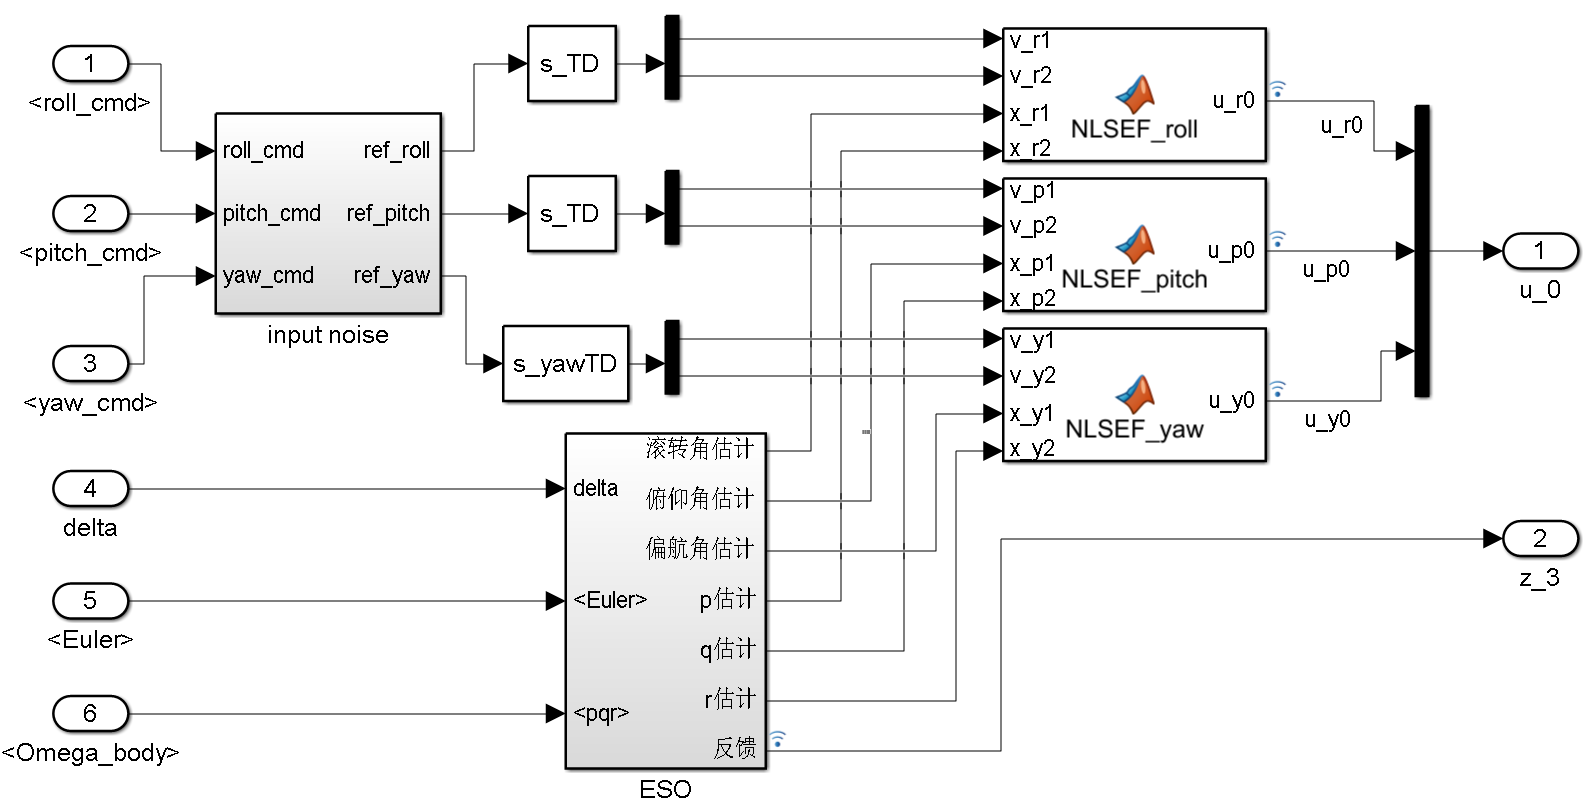
\includegraphics[scale=0.36]{Fig/Fig_Controller.png}
	\caption{\label{fig_controller_simulink}ADRC控制器仿真}
\end{figure}
\section{本章小结}
本章简要阐述了PID控制的诸多不足,结合所研究对象的特性,考虑使用ADRC对涵道无人机进行姿态控制。第二节介绍了ADRC的主要思想,紧接着讨论了其收敛性条件并不加证明地给出几条定理。最后,第三节针对涵道无人机的姿态系统设计了ADRC控制器,应用第二节给出的定理说明了所设计的自抗扰控制收敛,并借助MATLAB$^\circledR$/Simulink$^\circledR$搭建控制器仿真。








